\documentclass[twocolumn, a4paper]{article}
\usepackage{graphicx}
\usepackage{amsmath, amsthm, amssymb}
%%% Code environment
\usepackage{listings}
\usepackage{courier}
\usepackage{xcolor}
\definecolor{commentsColor}{rgb}{0.497495, 0.497587, 0.497464}
\definecolor{keywordsColor}{rgb}{0.000000, 0.000000, 0.635294}
\definecolor{stringColor}{rgb}{0.558215, 0.000000, 0.135316}
\lstset{
	basicstyle=\ttfamily\small,                       %% the size of the fonts that are used for the code
	breakatwhitespace=false,                          %% sets if automatic breaks should only happen at whitespace
	breaklines=true,                                  %% sets automatic line breaking
	frame=tb,                                         %% adds a frame around the code  
	commentstyle=\color{commentsColor}\textit,        %% comment style
	keywordstyle=\color{keywordsColor}\bfseries,      %% keyword style
	stringstyle=\color{stringColor},                  %% string literal style
	numbers=left,                                     %% where to put the line numbers; possible values are               (none, left, right)
	numbersep=5pt,                                    %% how far the line-numbers are from the code
	numberstyle=\tiny\color{commentsColor},           %% the style that is used for the line numbers
	showstringspaces=false,                           %% underline spaces within strings only
	tabsize=2,                                        %% sets default tabsize to 2 spaces
	language=[Sharp]C
}
%%% Document
\begin{document}
\title{Exponential function}
\author{Wikipedia}
\maketitle
\section*{Introduction}
The exponential funtion is a mathematical function denoted by $f(x)=\textit{exp}(x)$ or $\textit{e}^x$. The real exponential function $\textit{exp}: \mathbb{R} \rightarrow \mathbb{R}$ can be characterized in a variety of equivalent ways. It is commonly defined by the following power series:
\begin{align}\label{exp-def}
	\textit{e}^x &=\sum_{k=0}^{\infty} \frac{x^k}{k!} \\
	&= 1 + x + \frac{x^2}{2} + \frac{x^3}{6} + \frac{x^4}{24} + \dots
\end{align}
\section*{Implementation}
The exponential function has been implemented with the following code:
\begin{lstlisting}
static double ex(double x) {
	if(x<0) return 1/ex(-x);
	if(x>1.0/8) return Pow(ex(x/2),2);
	return 1+x*(1+x/2*(1+x/3*(1+x/4*(1+x/5*(1+x/6*(1+x/7*(1+x/8*(1+x/9*(1+x/10)))))))));
	}
\end{lstlisting}
This implementation exhibits a recursive behavior where the last statement is the power series from \eqref{exp-def} with $k=10$ and this is the base case. The two lines above the base case are cases that successively reduces towards the base case. The first line returns 1 divided by the function itself with argument -x, such when a negative x value is passed to the function it gives $\frac{1}{\textit{e}^x}$. The second line basically says return $\left(\textit{e}^{x/2}\right)^2 = \textit{e}^x$, which is the function itself, but because of the x/2 argument, the case will successively reduce to the base case. If the second line just would be written as \textit{return ex(x);} then we would get a stack overflow exception, which means that the recursion would go on infinitely. This would happen since it would never reach the base case.\\
The above implementation is tested by making a plot and also by plotting some tabulated values as a reference. This can be seen in figure \ref{exp-graph}.
\begin{figure}[!h]
	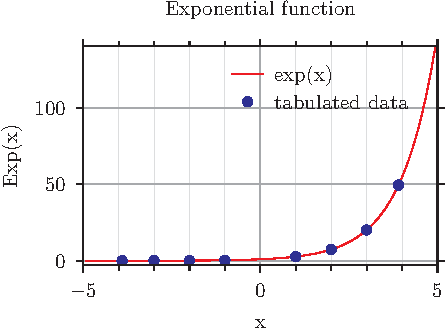
\includegraphics{exp_pyx.pdf}
	\label{exp-graph}
\end{figure}

\end{document}
